% Template for ISBI paper; to be used with:
%          spconf.sty  - ICASSP/ICIP LaTeX style file, and
%          IEEEbib.bst - IEEE bibliography style file.
% --------------------------------------------------------------------------
\documentclass{article}
\usepackage{spconf,amsmath,graphicx}
\usepackage{cite}


% Example definitions.
% --------------------
\def\x{{\mathbf x}}
\def\L{{\cal L}}

% Title.
% ------
\title{One-Shot Lung Segmentation based on Learned Transformations in a Cross-Dataset Scenario
  }

  %  Data Argumentation via learned transformations for One-Shot Lung Segmentation
%
% Single address.
% ---------------
% \name{Author(s) Name(s)\thanks{Thanks to XYZ agency for funding.}}
% \address{Author Affiliation(s)}
%
% For example:
% ------------
%\address{School\\
%	Department\\
%	Address}
%
% Two addresses (uncomment and modify for two-address case).
% ----------------------------------------------------------
% \twoauthors
%  {Qiuli~Wang,Zhihuan~Li, Xiaohong~Zhang\sthanks{This work was partially supported by the National Natural Science Foundation of China (Grant No. 61772093), the Chongqing Major Theme Projects (Grant No. cstc2018jszx-cyztzxX0017). Qiuli~Wang and Zhihuan~Li contribute equally to this paper.}}
% 	{School of Big Data \& Software Engineering \\Chongqing University \\ Chongqing, 400000, China }
%  {Chen~Liu}
% 	{Radiology Department \\ The First Affiliated Hospital of \\Army Medical University \\ 400032, Chongqing, China}
%
% More than two addresses
% ----------------------- $^{\star}$ $^{\ddagger}$
\name{Qiuli~Wang, Zhihuan~Li, Wei~Chen, Jiuquan~Zhang$^{\star}$, Hongqian~Wang, Chen~Liu$^{\dagger}$, Xiaohong~Zhang$^{\ddagger}$\sthanks{This work was partially supported by the National Natural Science Foundation of China (Grant No. 61772093), the Chongqing Major Theme Projects (Grant No. cstc2018jszx-cyztzxX0017).}}

\address{$^{\ddagger}$School of Big Data \& Software Engineering, Chongqing University, Chongqing, 400044, China \\
$^{\dagger}$The First Affiliated Hospital of Army Medical University, Chongqing, 400032, China\\
$^{\star}$Chongqing University Cancer Hospital \& Chongqing Cancer Institute, Chongqing, 400030, China}
%
\begin{document}
%\ninept
%
\maketitle
% Labeling CT scans is a time-consuming task and different datasets acquired from different types of CT equipment may have various data characteristics.
\begin{abstract}
    Lung segmentation on CT  is a core step for many studies on pulmonary diseases. Supervised methods have attained state-of-the-art accuracy; however, these methods heavily rely on supervised training with large labeled datasets.
    In this study, we present a framework for one-shot lung segmentation based on learned spatial and density transformations in a cross-dataset scenario.
    Our framework requires only one labeled CT scan (source scan), and transform this scan according to the target scans using spatial and density transformations, which learn the lung spatial deformation field and structural density based on CNNs. These target scans are not limited to the same dataset as the source scan, but can also come from another dataset or acquired from other types of CT equipment. Meanwhile, using the spatial transformation, we can generate labels for each transformed scans. Finally, we will train a supervised U-Net with generated labeled scans.
    Moreover, we design a multi-density MSE loss to improve transformations since the ribs are natural boundaries for the lungs.
    As far as we know, we are the first to segment lungs using the one-shot method. Our experiments demonstrate that our framework can achieve convincing results on VESSEL12 and clinical CT chest scans.

\end{abstract}
%
\begin{keywords}
One-Shot, Lungs, Segmentation, CT (Computed Tomography), U-Net
\end{keywords}
%
\section{Introduction}
\label{sec:intro}

Lung segmentation on CT (Computed Tomography) is a core step for many studies on pulmonary diseases. Supervised learning methods attain state-of-the-art accuracy, but these models have some common drawbacks.

First of all, these supervised methods heavily rely on labeled datasets. Labeling lungs on CT scans requires significant expertise and time, since one case of chest CT contains about 200 slices. As a result, public available lung CT datasets, like \cite{rudyanto2014comparing, yang2017data} are usually small. These datasets can not reflect the clinical diversity of lung structures.

Second, CT scans collected from different types of equipment vary in basic settings, which can cause different noise or image quality. As a result, the performances of the supervised models trained on the particular dataset are not stable on another dataset.
The drawbacks mentioned above have become limitations of clinical application for the supervised lung segmentation models.

In this study, we propose a framework for one-shot lung segmentation. Our method needs only one labeled chest CT scan from VESSEL12, and generate new scans with segmentation map according to the target scans, even if these target scans come from another dataset.

The process of our framework is shown in Fig.~\ref{transarti}.
\begin{figure*}[htbp]
    \centerline{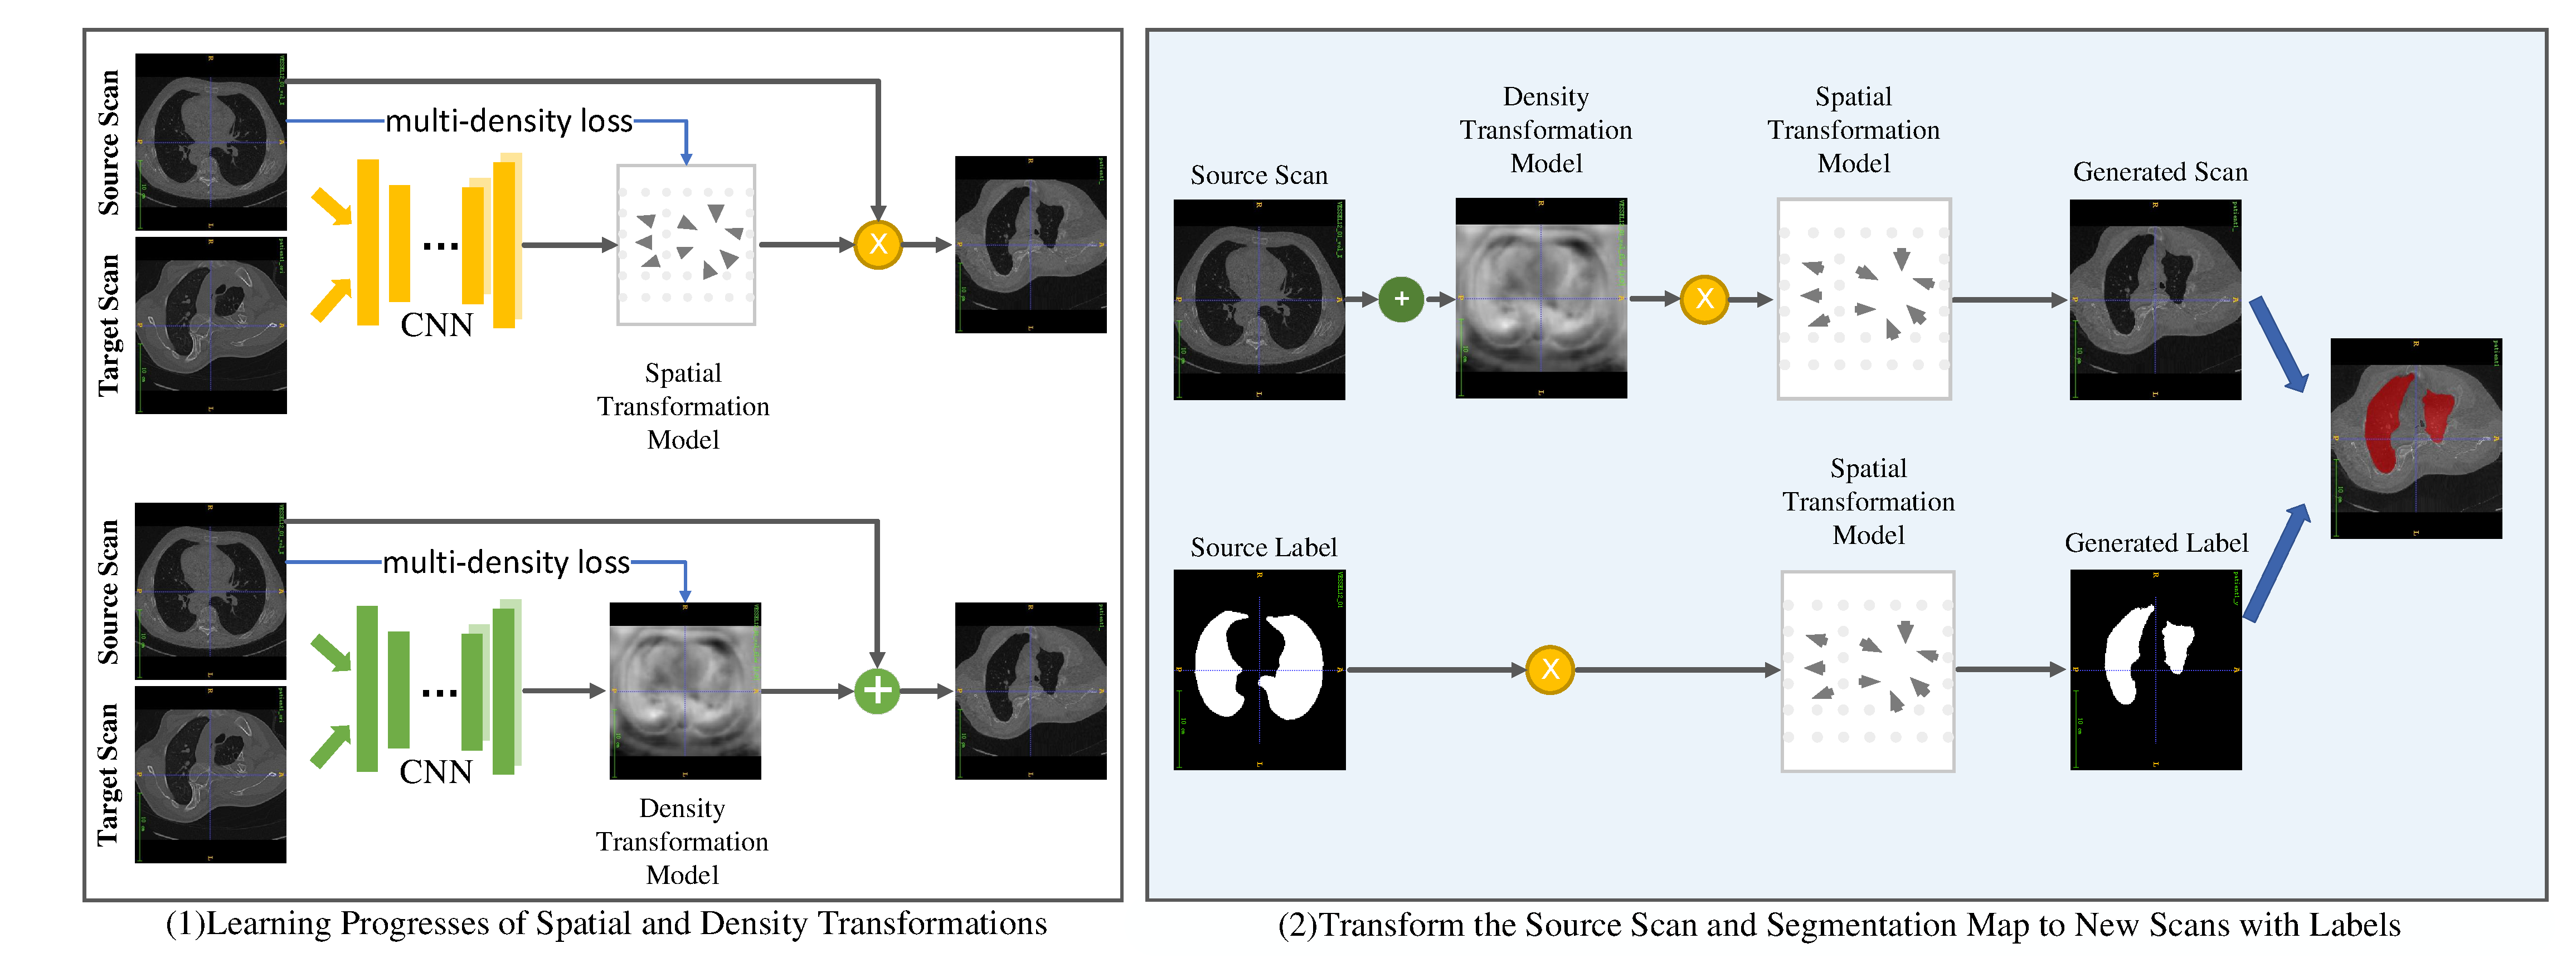
\includegraphics[width=180mm]{transarti2.pdf}}
    \vspace{-0.5cm}
    \caption{The overview of our framework. (1) The learning processes of spatial and density transformations. We use two separate U-Net models to learn the transformations, and use a multi-density MES loss to improve the transformation. (2) The process of transforming the source scan with segmentation maps to new labeled scans. Different from transforming a case, transforming a label only needs the spatial transformation.
    }
    \vspace{-0.3cm}
    \label{transarti}
    \end{figure*}
We first have a source scan from VESSEL12, which has segmentation maps. Second, we use two U-Net models to learn spatial and density transformations between source scan and target scans. Third, we apply spatial and density transformations to the source scan to synthesize new scans. Then, we apply spatial transformations to the segmentation map of the source scan to get segmentation maps for the generated new scans. Finally, we train a supervised U-Net with these generated labeled scans.


The major contributions of this paper can be summarized as follows:
(1)We propose a framework for one-shot lung segmentation based on learned transformations. The whole framework needs only one labeled example. (2)We design a multi-density MSE loss to improve the transformations, so that we can take advantages of natural boundaries of lungs, i.e., ribs. (3)We evaluate our framework on VESSEL12 and clinical CT scans, and our method shows good generalization ability and effectiveness in a cross-dataset scenario.

\section{Related Work}
\label{sec:related}
\subsection{Lung Segmentation}
Lung segmentation is a basic task for many studies on pulmonary diseases. Diverse works aimed to segment the lung region using different and combined techniques, that goes through region-growing, border analysis, shape and probabilistic models, and recently deep learning approaches. Most of them are supervised models, and they attain state-of-the-art accuracy. 

Traditional methods (i.e., region-growing, border analysis and so on) are mature but have some disadvantages in medical image segmentation \cite{adams1994seeded, kass1988snakes, canny1987computational}.
However, a study in \cite{soliman2016accurate} achieved $99.00 \pm 0.5$ in Dice sources using adaptive appearance-guided shape modeling.

Deep learning methods, especially CNN models (Convolutional Neural Network) have been widely used to segment medical images, like U-Net \cite{ronneberger2015u}, H-DenseUNet \cite{li2018h}, 3D U-Net \cite{cciccek20163d} and so on. 
Study in \cite{alves2018extracting} extract lungs from CT images using fully convolutional networks. Their method achieved $99.19 \pm 0.47$ in Dice Scores on VESSEL12, which is the state-of-art.
Most deep learning methods heavily rely on labeled datasets. However, public available big-scale medical datasets are very rare, which also limits the clinical application of supervised deep learning models.

\subsection{Spatial Transformer Networks}
Spatial transformer networks \cite{jaderberg2015spatial} and its variations have been used in a variety of image analyses, such as handwritten digits classification \cite{hauberg2016dreaming, learned2005data}, medical image registration, or data argumentation.
Guha~Balakrishnan et al. \cite{balakrishnan2019tmi} proposed VoxelMorph, a unsupervised learning-based method, to learn spatial transformations and finish the task of registration between brain MRI 3D volumes. Amy~Zhao et al. \cite{zhao2019data} proposed a method based on spatial and appearance transform. This model used two U-Net models to implement data argumentation using learned transformations for one-shot brain MRI image segmentation. 

\section{MATERIALS AND METHODS}
\label{sec:materials}
\begin{figure*}[htbp]
    \centerline{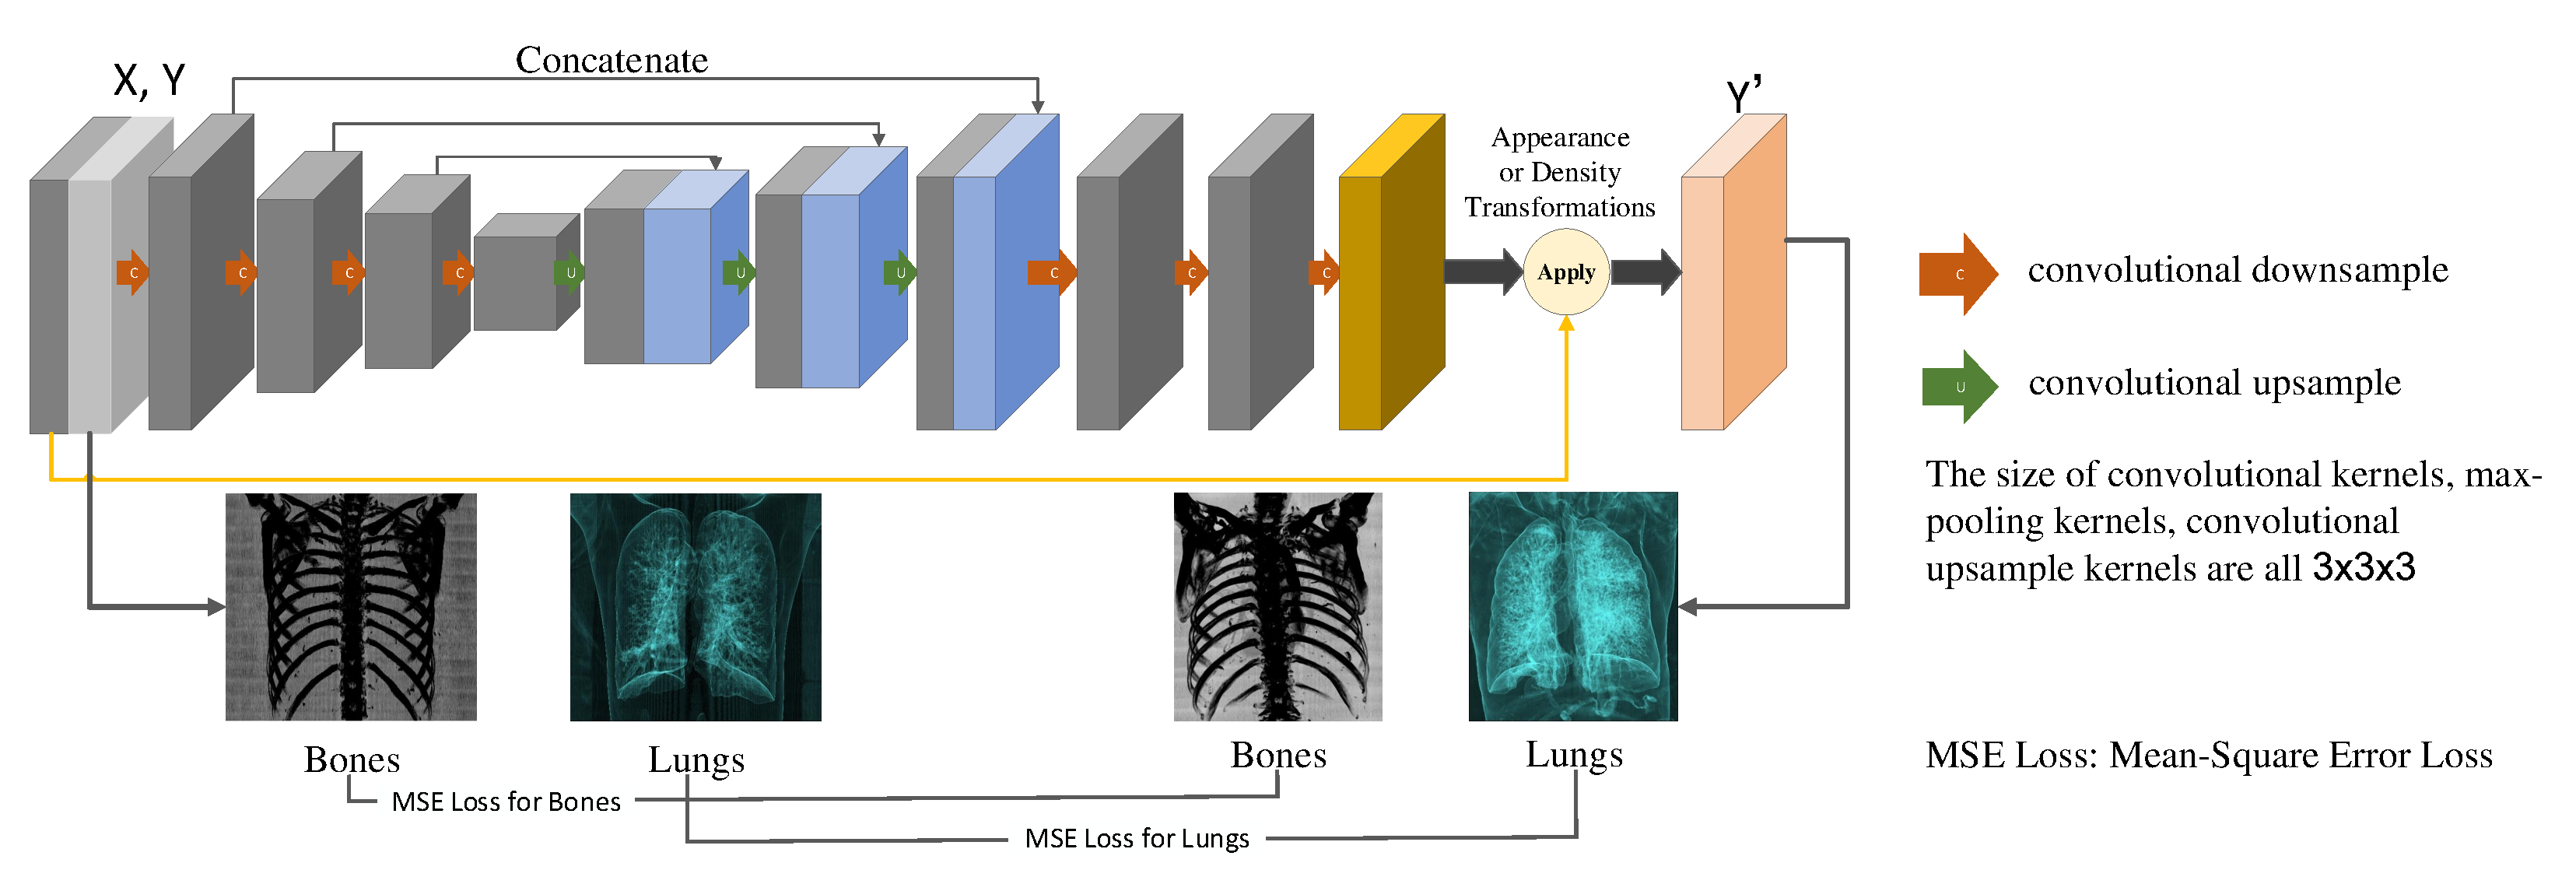
\includegraphics[width=180mm]{unet.pdf}}
    \vspace{-0.3cm}
    \caption{The structure of U-Net. X and Y indicates source scans and target scans. Y' indicates the generated results. U-Net models for spatial and density transformations are exactly the same. The loss function contains two parts: MSE for bones, and MSE for lungs. Bones like ribs are natural boundaries for lungs, which can help to improve the transformations.
    }
    \vspace{-0.3cm}
    \label{unet}
    \end{figure*}
\subsection{Datasets}
\label{dataset}
In this study, we use two datasets, which contain a total of 110 cases.
The first dataset is VESSEL12 \cite{rudyanto2014comparing}, which was proposed for the evaluation of both semi and automatic methods for lungs’ blood vessel segmentation in CT scans. A total of 20 scans are available for testing. Scans have an average of 432 slices, and each scan contains segmentation maps for lungs. This dataset is available online\footnote{https://vessel12.grand-challenge.org/}.
The second dataset is a clinical private dataset, which is collected from the Radiology Department, The First Affiliated Hospital of Army Medical University. A total of 90 scans are included. Since it is a private dataset collected directly from the clinic, we don't have segmentation maps for each scan. The data we use has been reviewed and desensitized.

\subsection{Methods}
\label{methods}

We propose to improve one-shot lung CT segmentation by generating new training chest CT with segmentation maps in a semi-supervised learning framework. The key point of this framework is the learning of spatial and density transformations.

We describe the differences between scans using a combination of spatial and density transformations. 
Let $T(\cdot)$ denote a transformation from one CT scan to another as a combination of a spatial transformation $t_s(\cdot)$ and a density transformation $t_d(\cdot)$. Then we have $T(\cdot)=t_s(t_d(\cdot))$. 
We model our spatial and density transformations as follows:
\begin{equation}
    t_s(x)=x\circ\mu,\qquad\qquad\mu=g\theta_s(x,y)
\end{equation}
\begin{equation}
    t_d(x)=x+\rho,\quad\rho=h\theta_d(x,y\circ\mu^{-1})
\end{equation}
We define the deformation function $\mu=id+u$, where id is the identity function, $u$ is a smooth voxel-wise displacement field. 
We use $x\circ\mu$ to denote the application of the deformation $\mu$ to $x$, and $x+\rho$ to denote the application of the deformation $\rho$ to $x$.
In our study, $x$ is the source scan. $g\theta_s$ and $h\theta_d$ are trainable parameters for two transformation models. $\mu^{-1}$ indicates the reverse deformation. 

The parameters of framework are optimized as follows:
\begin{align*}
    L(x,y^{(i)},\mu^{(i)},\mu^{-1(i)},\rho^{(i)},c_x)=\qquad\qquad\\L_{sim}((x+\mu^{(i)})\circ\mu^{(i)}, y^{(i)})+\lambda L_{smooth}(c_x,\rho^{(i)})
\end{align*}
\begin{align*}
    L_{sim}((x+\mu^{(i)})\circ\mu^{(i)}, y^{(i)})=\quad\\\sigma_1L_{sim}((x_{bone}+\mu^{(i)})\circ\mu^{(i)}, y_{bone}^{(i)})+\\\sigma_2L_{sim}((x_{lung}+\mu^{(i)})\circ\mu^{(i)}, y_{lung}^{(i)})
\end{align*}
where $i$ indicates the $i$-th target scan. $L_{smooth}$, which is calculated as $(c_x,\rho)\nabla\rho$, is a smoothness regularization function based on the segmentation map of the source scan.
$L_{sim}$ is mean squared error for the image similarity loss.
In \cite{zhao2019data}, $L_{sim}$ only calculated single loss of image similarity loss. However, their study was about brain segmentation. The spatial structures of the brain have a much smaller range than that of the lungs, so the single loss of image similarity cannot meet the requirements of lung transformations. In our study, $L_{sim}$ is a multi-density loss, which contains losses for both CT images and bone structures. We use bone structures to improve the transformation since bones like ribs are the natural boundaries for lungs. $\lambda$, $\sigma_1$ and $\sigma_2$ are parameters, which can be optimized by back-propagation algorithm.
Both density and spatial transformations are learned by separate U-Nets, as shown in Fig.~\ref{unet}.

In Fig.~\ref{generatedata}, we show two generated cases with its target cases. We can see that the generated scans are very similar to target scans, and the generated segmentation maps can cover the lung regions well.

\begin{figure}[htbp]
\centerline{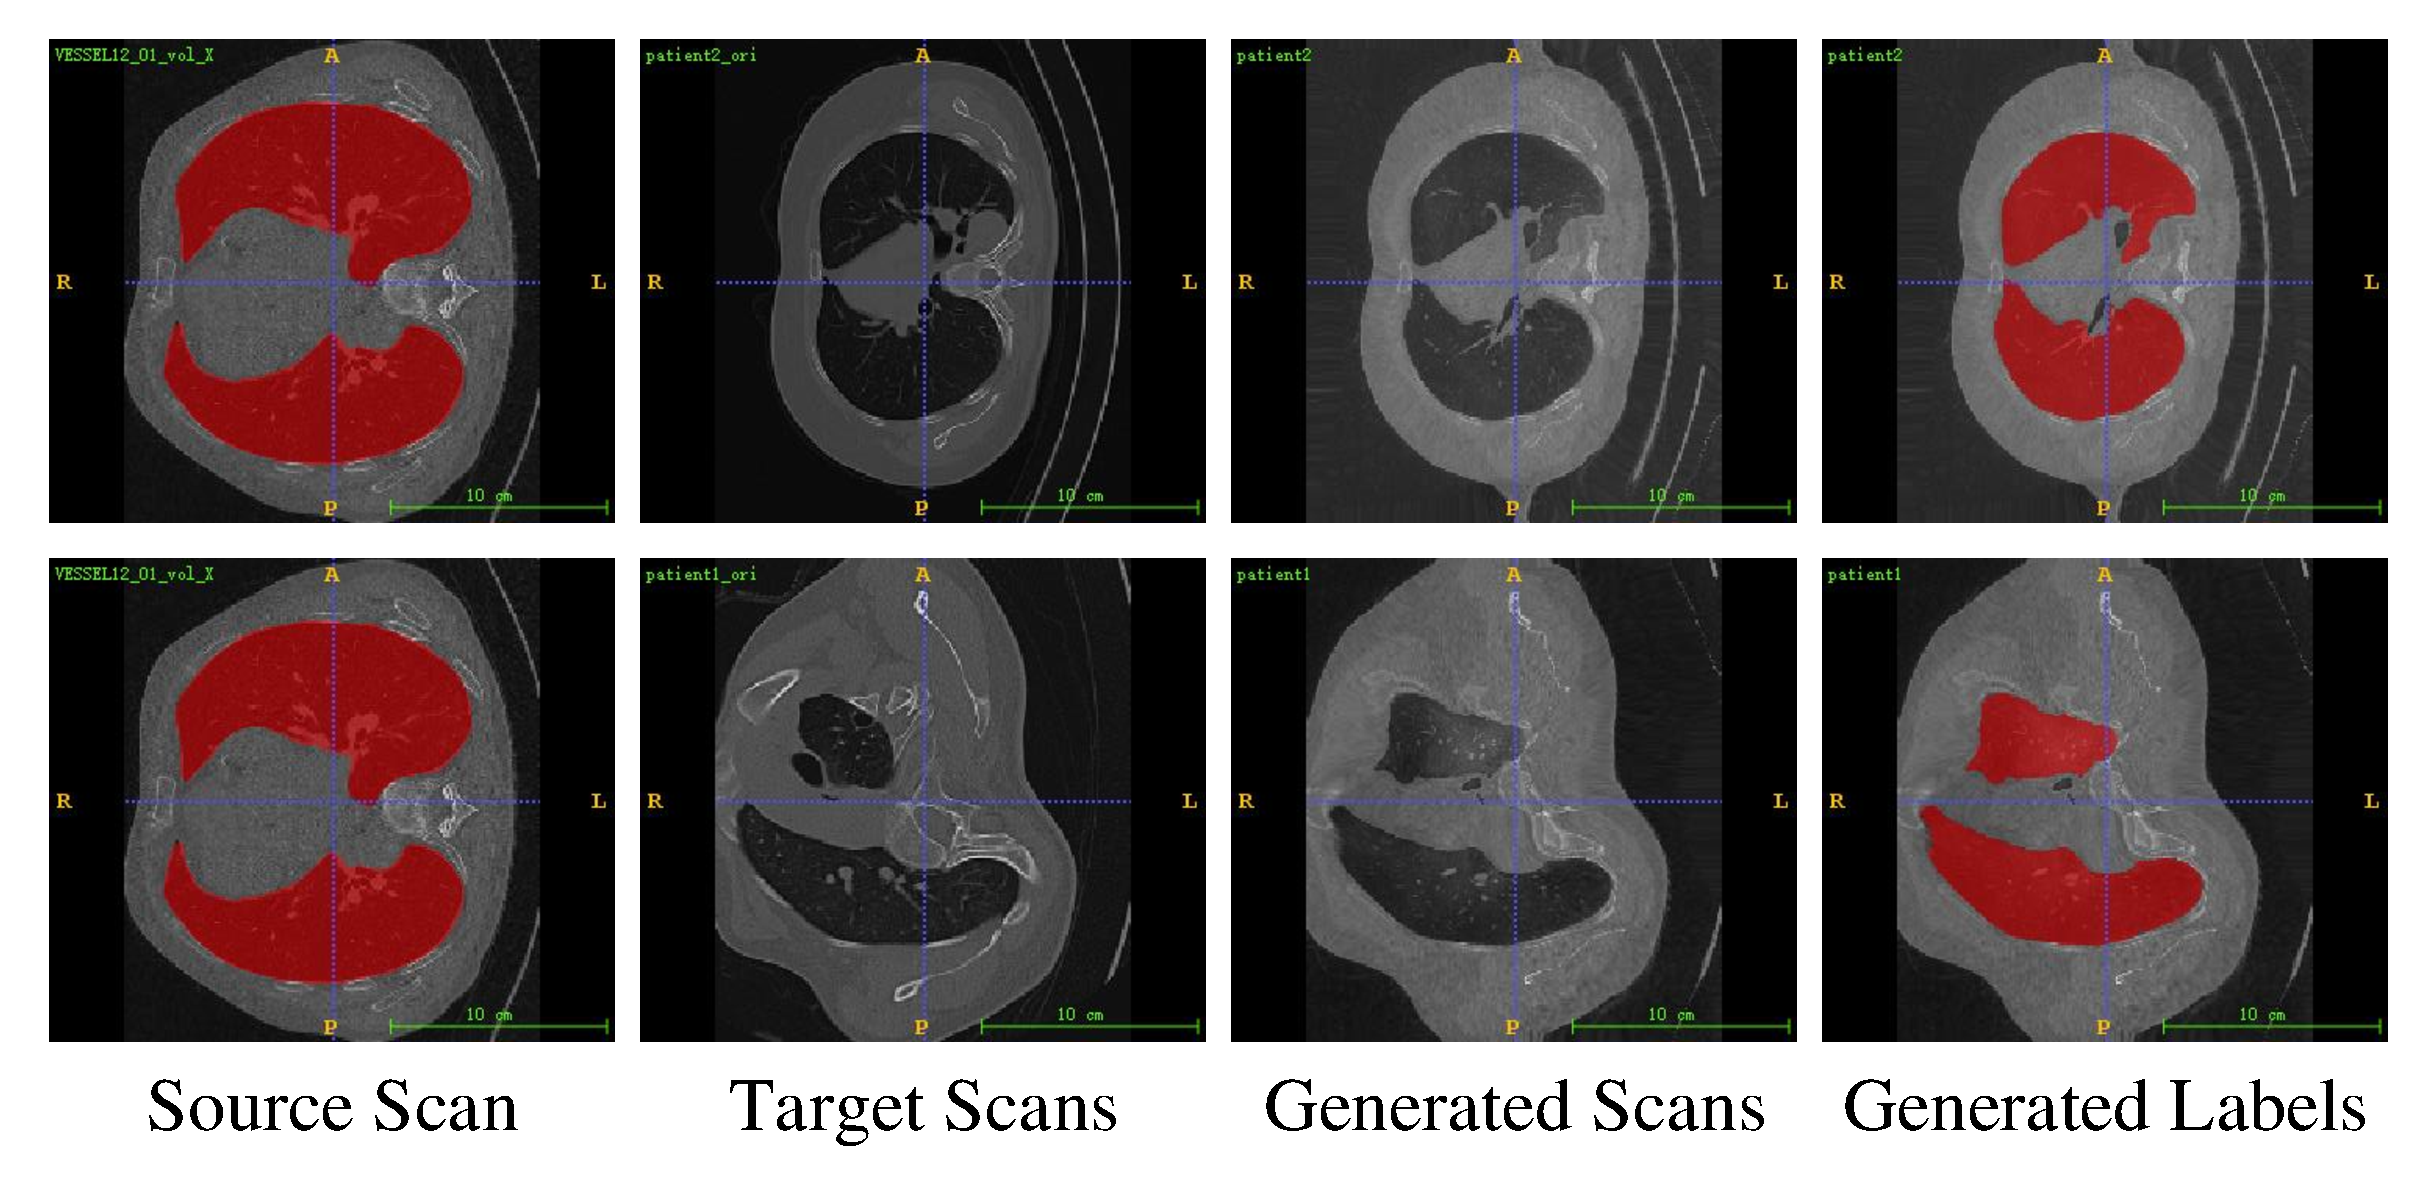
\includegraphics[width=90mm]{generatedata.pdf}}
\vspace{-0.5cm}
\caption{Comparisons between the source scan, target scans, generated scans and generated labels. The generated scans are similar to target scans, but still keep some features from the source scan. The generated segmentation maps can cover the lung regions well.
}
\vspace{-0.3cm}
\label{generatedata}
\end{figure}

\section{Experiments}
\label{sec:experiments}
In this section, we have conducted several experiments to analyze our model in detail. 
In the first part of the experiments, we quantitatively analyze the performance of our framework in a cross-dataset scenario. This part of the experiments is carried on with VESSEL12 since VESSEL12 provides segmentation maps for each scan so that we can calculate Dice Scores.
In the second part of the experiments, we verify the performance of our framework on clinical data. 
Due to the shortage of labeled data, we cannot quantitatively analyze segmentation results in this part, so that we invite 2 radiologists to give subjective judgments on segmentation results.

There are not many requirements for the selection of the source scan, except that the selected source scan needs a clear view of lungs and healthy bone structures.

\subsection{Results on VESSEL12}
\label{subsec:vessel}
In this section, we experimentally quantitative analyze the performances of our framework on VESSEL12 in the scenario of cross-dataset. Due to the shortage of labeled data, we only use VESSEL12 for evaluation, except the source scan. The target scans are collected from clinic.

In this section, we conduct two experiments.
First, we pick one case and its segmentation maps as source case, and generate 60 new cases using 60 clinical cases as our training set, then we train a U-Net(Ours) with these cases, and test the performance of this U-Net(Ours) on VESSEL12.
Second, we train a U-Net(One Scan) with only one segmented case (i.e., the source case) and test the performance of this U-Net(One Scan) in the same way. 

Experiments' results are listed in Table.~\ref{vesselres}. We use Dice Scores (DSC) \cite{dice1945measures} to evaluate the performances of segmentation results. According to Table.~\ref{vesselres}, supervised methods have achieved very convincing results. The state-of-the-art has achieved a Dice Score of 99.19. The U-Net trained with only labeled scan form VESSEL12 achieves an average Dice Score of 91.69. The U-Net trained with generated scans achieves 96.31, which is 2.88 lower than the state-of-the-art. Considering our method requires only one segmented scan, our results are quite convincing and there is a lot of room for improvement if we have more labeled scans and improve the transformations.

\begin{table}[htbp]
    \vspace{-0.5cm}
    
    \caption{Comparison among Different Methods}
    \begin{center}
    \begin{tabular}{c|c|c}

    \hline
    \textbf{\textit{Methods}} & \textbf{\textit{Training Data}}& \textbf{\textit{DSC}}\\
    \hline
    Soliman et al. \cite{soliman2016accurate} & VESSEL12 & $99.00$ \\
    Alves et al. \cite{alves2018extracting} & VESSEL12 & $99.19$ \\
    \hline
    U-Net(One Scan) & One Scan from VESSEL12 & $91.69$ \\
    U-Net(Ours) & Generated & $96.31$ \\
    \hline

    \end{tabular}
    \end{center}
    % \footnotesize{LW: Lung Window Image, HA: High Attenuation Image, LA: Low Attenuation Image, TC: Three-Channel Image}

    \vspace{-0.3cm}
    \label{vesselres}
    \end{table}

Moreover, we observe that some particular scans with severe diseases are difficult to segment. For example, our method only achieves a Dice Score of 91.44 on the 17-th scan of VESSEL12, which lowers the average score. This is because the 17-th scan of VESSEL12 has lung diseases and causes density changes in lungs. That would be very helpful if we can get more labeled scans that have severe diseases.

\subsection{Results on Clinical Data}
\label{subsec:clinical}
\begin{figure}[t]
    \centerline{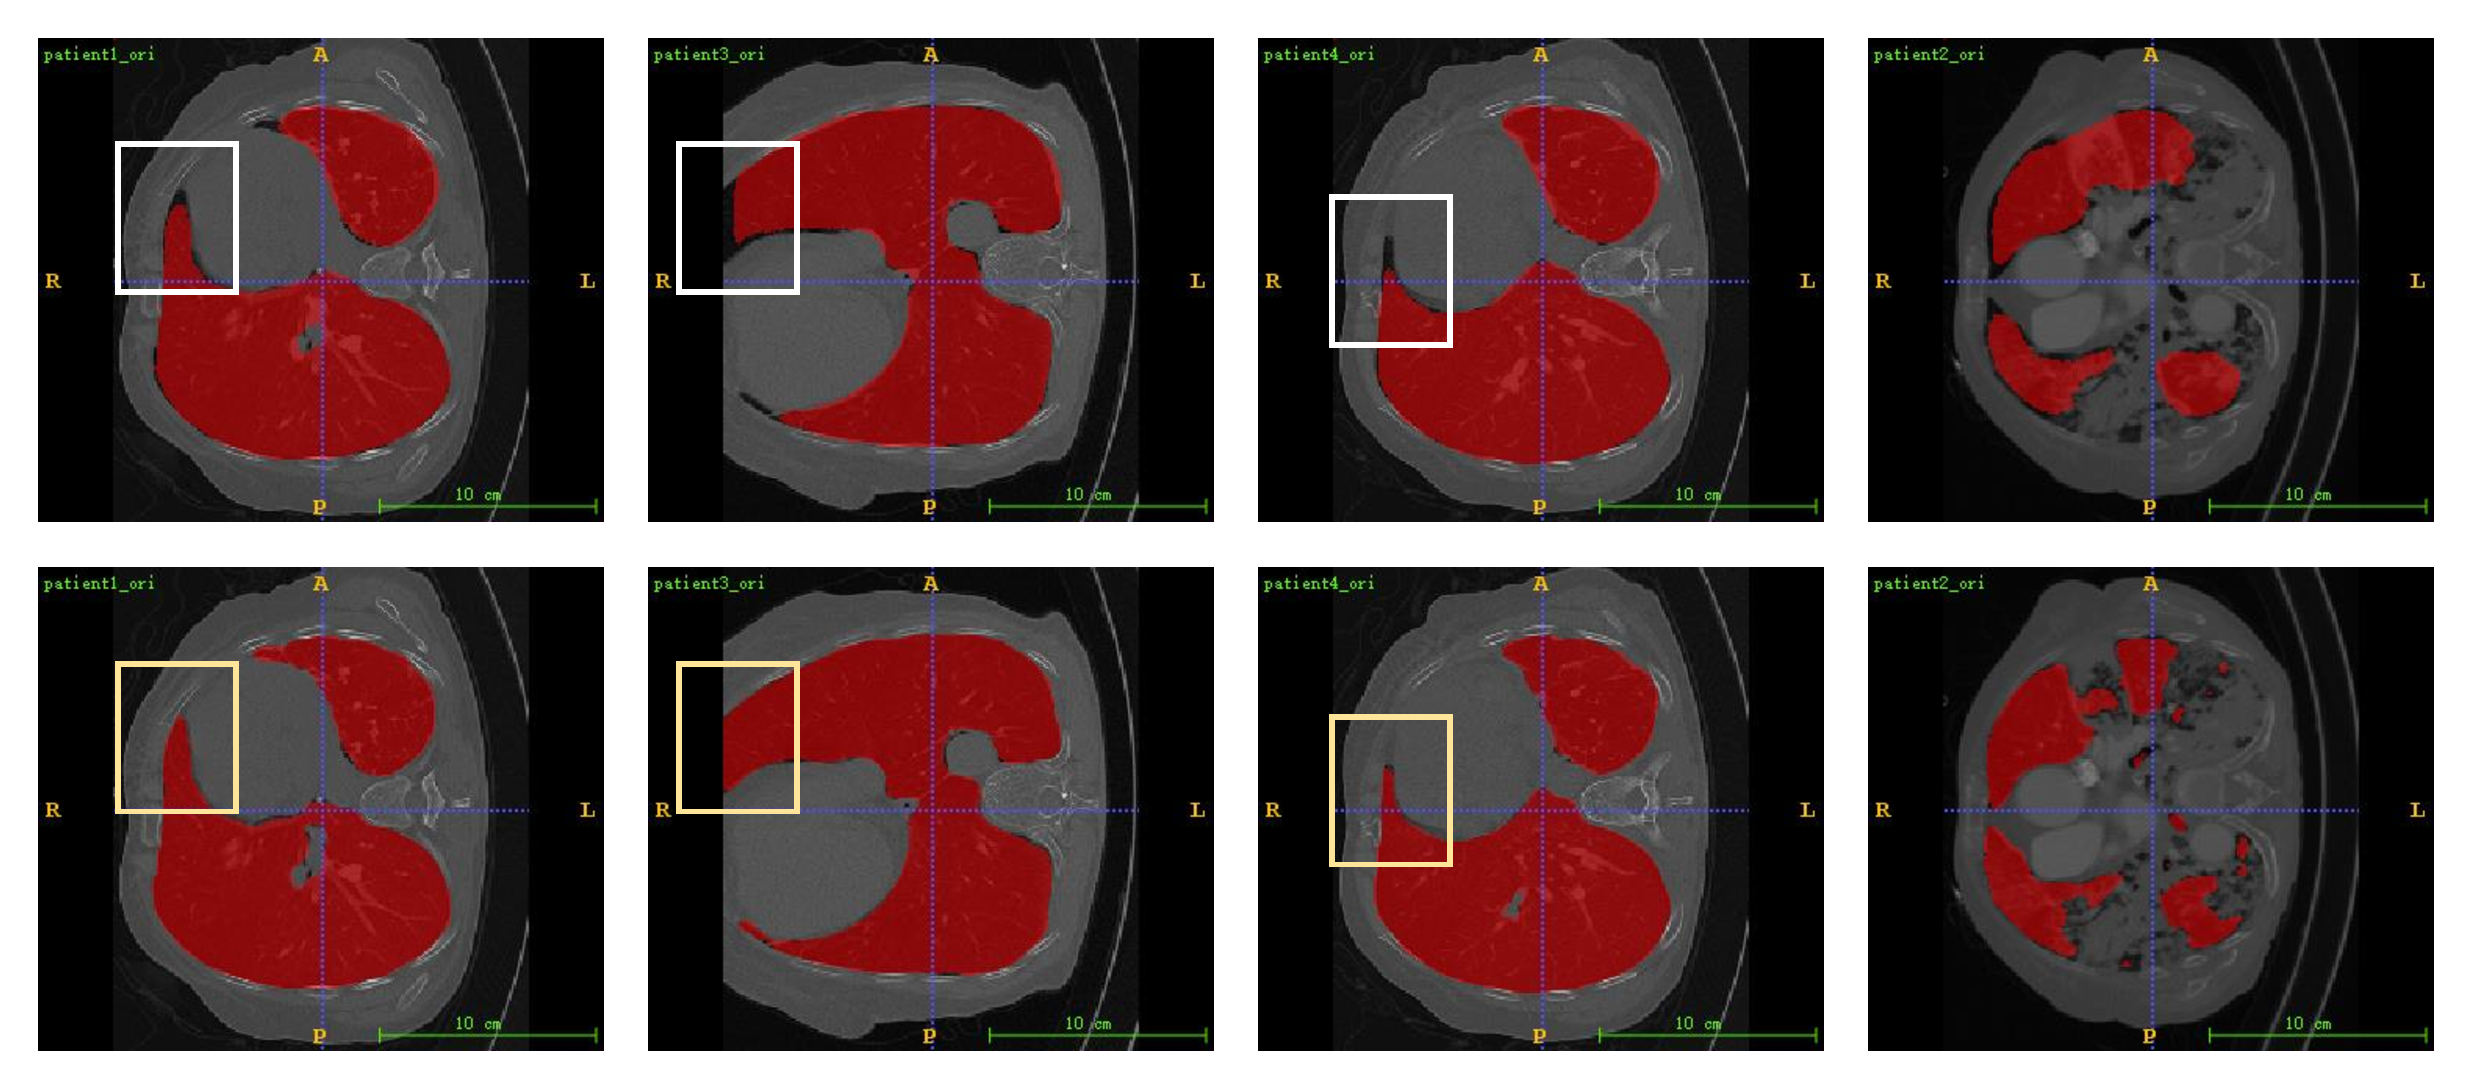
\includegraphics[width=90mm]{lungs.pdf}}
    \vspace{-0.5cm}
    \caption{The top row shows the segmentation results generated by a U-Net trained by VESSEL12. The bottom row shows the segmentation results generated by a U-Net trained by generated scans. 
    }
    \vspace{-0.3cm}
    \label{lungs}
    \end{figure}
In this section, we analyze the performances of our model on clinical data. We got 90 cases of chest CT, 60 cases are used to generate new data with labels, 30 cases are used to verify the segmentation results. Due to the shortage of labels of the private dataset, we invite two radiologists to give subjective judgments on segmentation results.

We conduct two experiments in this section.
First, we train a U-Net(VESSEL12) with all VESSEL12 data, then test this model on the testing set (30 cases).
Second, we use the source case with segmentation maps (the same as section~\ref{subsec:vessel}) and generate 60 new cases with segmentation maps. Then we train a U-Net(ours) and test this model one the 30 testing cases.

Experiments demonstrate that our method can improve the performance of U-Net. Fig.~\ref{lungs} clearly shows that U-Net trained with our scans has a better performance, especially in these narrow regions (areas in rectangles). However, both models perform worse when the lungs have severe lung diseases (the last column).

According to two radiologists, in 30 testing cases, our framework has a better performance in 21 cases. Then both methods perform worse on 6 cases, and both segment lungs well on the left 3 cases.
We further investigate 6 cases which are difficult to segment. We find that these 6 cases all have severe lung diseases, which lead to great changes in lung density or lung structures. 

In a word, using generated scans can improve the performances of segmenting narrow lung regions and healthy cases. However, since we don't have enough labeled scans which have severe diseases, both models have difficulty in segmenting lungs with severe diseases.

\section{Conclusion}
\label{sec:discussconclusion}
In this work, we propose a framework for one-shot lung segmentation based on density and spatial transformations in a cross-dataset scenario. Our framework allows the supervised model to have a better performance using only one labeled case. Moreover, our framework provides a solution when we don have enough labeled data.

However, we only use one labeled source scan in our study, and it is very difficult to generate scans that can cover lungs with large changes like density changes or shape changes. This problem limits the effect of our framework. Our future work will focus on using diversify source scans and improve the quality of generated scans.

% References should be produced using the bibtex program from suitable
% BiBTeX files (here: strings, refs, manuals). The IEEEbib.bst bibliography
% style file from IEEE produces unsorted bibliography list.
% -------------------------------------------------------------------------
\bibliographystyle{IEEEbib}
\bibliography{refs}

\end{document}
